\documentclass[9pt,twocolumn]{paper-template}
% Use the lineno option to display guide line numbers if required.
\usepackage{lipsum}
\usepackage{tabularx} % in the preamble
\usepackage{subcaption}
\usepackage{multirow}
\templatetype{twocolumn} % Choose template 
% {pnasresearcharticle} = Template for a two-column research article
% {pnasmathematics} %= Template for a one-column mathematics article
% {pnasinvited} %= Template for a PNAS invited submission

\title{A Review on Interacting Adaptive Processes Which Underlie Short-Term Motor Learning}

% Use letters for affiliations, numbers to show equal authorship (if applicable) and to indicate the corresponding author
\author[a]{MohammadAmin Alamalhoda}
\author[a]{Arsalan Firoozi} 
\author[a]{Mohammad khorshidi}
\affil[a]{Student, EE Department, Sharif University of Technology}

% Please add here a significance statement to explain the relevance of your work
\significancestatement{Multiple models have tried to simulate the motor skill acquisition but most of them fail in producing some of the features of motor skill learning. Here a model is introduced where demonstrates that within a timescale of minutes, two distinct fast-acting processes drive motor adaptation. One process responds weakly to error but retains information well, whereas the other responds strongly but has poor retention. This two-state learning system makes the surprising prediction of spontaneous recovery (or adaptation rebound) if error feedback is clamped at zero following an adaptation-extinction training episode.}

% Please include corresponding author, author contribution and author declaration information
\authorcontributions{Author contributions}
\equalauthors{\textsuperscript{1}All contributed equally to this work}

% Keywords are not mandatory, but authors are strongly encouraged to provide them. If provided, please include two to five keywords, separated by the pipe symbol, e.g:
\keywords{Motor learning, Multi-Rate Model, Memory of Errors} 

\begin{abstract}

Multiple models have tried to simulate the motor skill acquisition but most of them fail in producing some of the features of motor skill learning. Here a model is reviewed that within a timescale of minutes, two distinct fast-acting processes drive motor adaptation. One process responds weakly to error but retains information well, whereas the other responds strongly but has poor retention. This two-state learning system is capable of predicting spontaneous recovery (adaptation rebound) if error feedback is zeros. The results suggest that motor adaptation depends on at least two distinct neural systems that have different sensitivity to error and retain information at different rates. Also, the motor skill learning will be more if the changes in the environment are slow. In this view, motor memory is a memory of motor commands, acquired through trial-and-error and reinforcement. Here is shown that the brain controls how much it is willing to learn from the current error through a principled mechanism that depends on the history of past errors. 
\end{abstract}

\dates{This manuscript was compiled on \today}

\begin{document}

\maketitle
\thispagestyle{firststyle}
\ifthenelse{\boolean{shortarticle}}{\ifthenelse{\boolean{singlecolumn}}{\abscontentformatted}{\abscontent}}{}

% If your first paragraph (i.e. with the \dropcap) contains a list environment (quote, quotation, theorem, definition, enumerate, itemize...), the line after the list may have some extra indentation. If this is the case, add \parshape=0 to the end of the list environment.
\section*{Introduction}
\dropcap{R}elearning a previously unlearned stimulus-response relationship is faster than the initial learning in case of savings in the system \cite{main_paper}. Compensating the disturbance from the external environment or the motor system itself is called motor adaptation. Recent studies show savings in motor adaptation \cite{Kojima}. Also, better performance is reported by having no feedback trials between extinction and re-adaptation trials \cite{Kojima}. 
Until now, three models of trial-to-trial adaptation is proposed: Single state, Gain specific, and multi-rate. The single state model predicts the motor responses to disturbances and successfully assesses the pattern of generalization [\cite{Scheidt} - \cite{Donchin}]; But the problem is that this model is single-time constant adaptation and this leads to failure in other experiments like anterograde interference, rapid de-adaptation, and rapid downscaling. In the anterograde interference paradigm we have an initial learning block and then a de-adaptation block in which we expect to have lower performance and a slower time constant for the de-adaptation block [\cite{Bizzi} - \cite{Wolpert}]. A two-state model is suggested by Kojima et al. which can successfully model saving and washout of saving but fails for recovery of the initially adopted state in no feedback error block and also fails for described anterograde interference \cite{Kojima}.
In this report, we showed that the multi-time constant model proposed by Smith et al. can correctly model the motor response under different experiments and paradigms \cite{main_paper}. Herzfeld et al. also presented a model in which they showed that the brain decides how much to learn from a current error based on the history of previous errors \cite{mem_error}. This is also implemented and tested under different disturbances.\\


\section*{Results}
Figure \ref{fig:saving} shows simulations of the experimental paradigm that shows saving in eye saccade adaptation. The progress of motor output in learn, unlearn, and re-learn paradigms with three different models is simulated. Models are (1) a single-state, single-time-constant model, (2) a two-state, gain-specific model, and (3) a two-state, gain-independent, multi-rate model. All of these models give motor output as a function of the current motor state and the error of the last trial. The learning rules for these models are:

\begin{eqnarray*}
& (1)\;Single\;State:\\
& x(n+1) = Ax(n)+Be(n)
\end{eqnarray*}

\begin{eqnarray*}
& (1)\;Gain\;Specific:\\
&x_1(n+1) = min(0,[Ax_1(n)+Be(n)])\\
&x_2(n+1) = max(0,[Ax_2(n)+Be(n)])\\
&x = x_1+x_2
\end{eqnarray*}


\begin{eqnarray*}
& (1)\;Multi\;Rate:\\
& x_1(n+1) = A_fx_1(n) + B_fe(n)\\
& x_2(n+1) = A_sx_2(n) + B_se(n)\\
&x = x_1+x_2
\end{eqnarray*}

All of these models have error term ($e(n)$) because there is a difference between the motor output $x(n)$ and the state of the environment $f(n)$, so: $e(n) = f (n) - x(n)$.\\
As it can be seen in the results of the simulations (Figure \ref{fig:saving}), the single-state model can't reproduce saving, while both the gain-specific model proposed by Kojima et al. and the multi-rate model proposed by Shadmehr et al. can produce saving. Also, both of these models show decay in the amount of saving when null trials are inserted before the learning block which makes sense based on our intuition of the motor control processes. Because the internal states are different, both systems’ responses to the learning stimulus are altered. re-learning is faster than initial learning in the gain-specific model because both the up and down states can contribute to re-learning whereas only the upstate contributes to initial learning. In the case of the multi-rate model, re-learning is faster than initial learning because when re-learning starts, the
slow state is already biased towards re-learning, making re-learning more dependent on the fast state compared to initial learning.\\



\begin{figure*}[h!]
  \centering
    \includegraphics[width=\linewidth]{figures/figure1/Fig}
  \caption{\textbf{Simulations of Motor Adaptation Experiments That Show Savings}\\
  (A) Shows the model simulations of the experiment paradigm (Disturbance plot) which is plotted in black. (B) Shows a direct comparison of simulated performance in the initial learning and re-learning blocks.  (C) Shows the amount of savings found in simulation, as a function of the number of washout trials. The amount of savings is measured as the percent improvement in performance on the 30th trial in the re-learning block compared to the 30th trial in the initial learning block. 
}
  \label{fig:saving}
\end{figure*}


Although there are similarities in predictions of the gain-specific model and multi-rate model, there are differences in their internal states. It suggests that these models can evolve different motor adaptations through specific trials. Here we set up a test that a zero error paradigm (error-clamp) comes after the unlearning state, and the experiment becomes a learning, unlearning, and error clamp (Figure \ref{fig:error_clamp} A). In this case, the gain-specific and multi-rate models show different predictions about the evolution of motor output (Figure \ref{fig:error_clamp} A). In the gain-specific model, the forecast of the motor output following unlearning block remains at zero.
In contrast, the multi-rate model transiently rebounds the motor output during the learning block in the error-clamp paradigm instead of staying zero during this block. On the other hand, the multi-rate model transiently rebounds the motor output during the learning block in the error-clamp paradigm instead of remaining zero. The fast state of the multi-rate model keeps following the blocks very well, but the slow state keeps tracking the learning block's motor output during the unlearning state and helps the model to rebound the motor output of the learning state transiently. Here we test another trial in which there is a re-learning block after the error-clamp state (Figure \ref{fig:error_clamp} C). With the multi-rate model, the rebounding in the error-clamp state accelerates re-learning and demonstrates the saving in this case, while the gain-specific model is unable to demonstrating this (Figure \ref{fig:error_clamp} C).
We then try to use a washout trial instead of the error-clamp paradigm, where the output is zero instead of the error (Figure \ref{fig:error_clamp} B). We can see that after de-adaptation, the motor output of the single state model is negative for a short time, but after that, it remains at zero. For gain-specific model, the same thing happens but the difference is the time of being negative for the motor output and it is more negative for the gain-specific model. The output of the multi-rate model is a little bit different from the error-clamp paradigm. The rebound effect can be seen here, too; But the peak of the rebound is less than the error-clamp paradigm (Figure \ref{fig:error_clamp} B). The reason for the differences is that the f(x) is zero instead of e(x), and it leads to differences in the peak values. We do it also for the second stimulation in the last part. Also, we switched the error clamp with the washout paradigm (learning, unlearning, re-learning) (Figure \ref{fig:error_clamp} E). The difference between the output of the single-state model with error-clamp and washout paradigm is just a little bit of being negative for a short while after unlearning block. The difference between outputs of the gain-specific model in two trials is just like the Single state model and there is a undershoot after the unlearning block. In contrast, the differences between the outputs of the multi-rate model are in the peak of the rebound, and a little undershoot after unlearning block. Also, a difference between the two fast states can be seen (Figure \ref{fig:error_clamp} E).



\begin{figure*}[h!]
  \centering
    \includegraphics[width=\linewidth]{figures/figure3/Fig}
  \caption{\textbf{ Simulation of Motor Adaption in Error-clamp and Washout Paradigm}\\
The columns are different models, from left to right: single-state model, Gain-specific model, and multi-rate model.(A) The first two models just follow the baseline after the unlearning block and in the error-clamp paradigm. But in the multi-rate model for the error-clamp paradigm, we can see a transient rebound in motor output and in the direction of the motor output displayed in the initial learning block, resulting in spontaneous recovery.
(B) Paradigm for simulated washout experiment, where an error-clamp block in figure 2A is replaced by a washout block. The washout block is where the output is zero, not the error. The columns are the same as in (A). The difference between this section and (A) is the undershoot in single-state and gain-specific model after unlearning paradigm. In the multi-rate model, the peak of the transient rebound is less than in (A). Also, we can see an undershoot after unlearning block.
(C) Paradigm for error-clamp/re-learning experiment. Here there is a re-learning block coming after the error-clamp block. The columns are like (A). The multi-rate model predicts the performance at the start of the re-learning block better than the baseline. The other two models start from the baseline at the start of the re-learning block. 
(D) Paradigm for simulated washout/re-learning experiment. The paradigm is just like (C), but the error-clamp block is replaced by washout, where the output f(x) is zero, not the error.
}
  \label{fig:error_clamp}
\end{figure*}


\begin{figure}[h!]
  \centering
     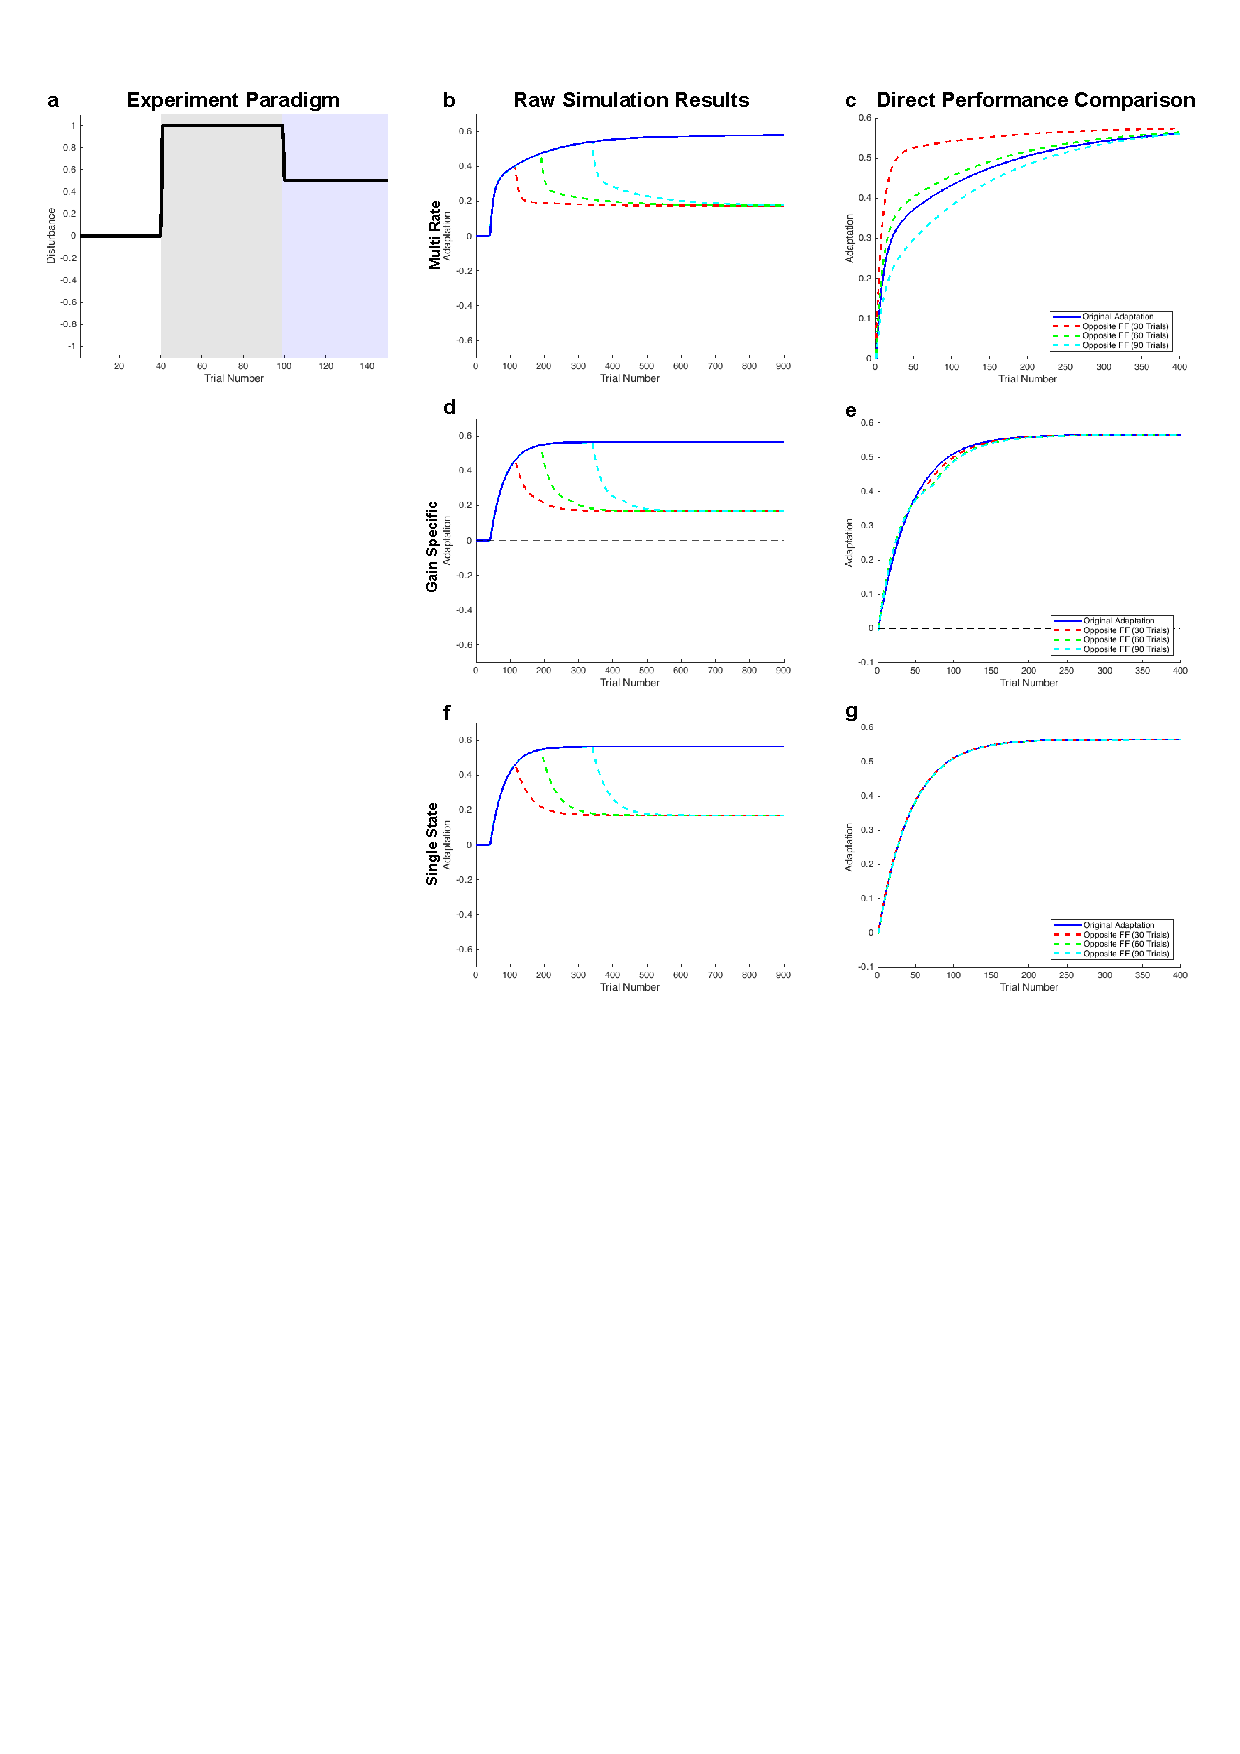
\includegraphics[width=\linewidth]{figures/Fig6}
  \caption{\textbf{Anterograde Interference Simulation}\\(A)  Experiment Paradigm. (B, D, F) Raw simulation results of multi-rate model, gain-specific model, and Single State model. Blue: initial adaptation. Red, Green, Cyan: secondary adaptation after 30, 60, and 120 initial adaptation trials. (C, E, G) Direct performance comparison of multi-rate model, gain-specific model, and Single State model. In this column, learning curves are shifted and scaled so that the desired performance is one. In this paradigm only the multi-rate model has a higher time constant in the initial adaptation compared to the time constant of de-adaptation; the single state model shows no change in the time constant and the gain-specific model shows a faster time constant for the secondary adaptation. Since we have a bias against the de-adaptation, it is expected to have a slower time constant in the second adaptation in the multi-rate model. And the results show that in the multi-rate model we get a slower time constant by increasing the number of adaptation trials. 
}
  \label{fig:Anterograde_Interference_Simulation}
\end{figure}


\begin{figure}[h!]
  \centering
     \includegraphics[width=\linewidth]{figures/Fig7}
  \caption{\textbf{Deadaptation Simulation}\\ (A)  Experiment Paradigm. (B, D, F) Raw simulation results of multi-rate model, gain-specific model, and Single State model. Blue: initial adaptation. Red, Green, Cyan: secondary adaptation after 30, 60, and 120 initial adaptation trials. (C, E, G) Direct performance comparison of multi-rate model, gain-specific model, and Single State model. In this column, learning curves are shifted and scaled so that the desired performance is one. In this paradigm, the multi-rate model and the gain-specific model show a faster rate of de-adaptation while the single-state model shows no changes in the rate. Also, it can be inferred that by increasing the number of adaptation trials, the rate of de-adaptation decreases. 
}
  \label{fig:Deadaptation_Simulation}
\end{figure}


\begin{figure}[h!]
  \centering
     \includegraphics[width=\linewidth]{figures/Fig8}
  \caption{\textbf{Down-Scaling Simulation}\\ (A)  Experiment Paradigm. (B, D, F) Raw simulation results of multi-rate model, gain-specific model, and Single State model. Blue: initial adaptation. Red, Green, Cyan: secondary adaptation after 30, 60, and 120 initial adaptation trials. (C, E, G) Direct performance comparison of multi-rate model, gain-specific model, and Single State model. In this column, learning curves are shifted and scaled so that the desired performance is one. In this paradigm, the multi-rate model shows the effect of having a faster time constant of adapting to a lower level of previously learned adaptation than de-adaptation to baseline. The gain-specific model shows somehow inverse effect.
}
  \label{fig:Down_Scaling_Simulation}
\end{figure}



It’s been reported that an initial motor adaptation has a faster time constant in comparison with subsequent adaptation for the oppositely directed stimulus. [\cite{Bizzi}, \cite{shadmehr_jn}, \cite{Wolpert}] We’ve tested the multi-rate model under different stimuli and the result clearly shows we have a faster time constant for the initial adaptation. 
The first stimulus is Anterograde interference which consists of a number of trials (In this case: 30, 60, and 120) as adaptation and 50 trials as de-adaptation (Figure \ref{fig:Anterograde_Interference_Simulation} A). In Figure \ref{fig:Anterograde_Interference_Simulation} B, the raw response of the multi-rate model is shown; Also, in Figure \ref{fig:Anterograde_Interference_Simulation} D and F, you can see the response of Gain-specific model and Single State model. By comparing the time constants of each model (Figure \ref{fig:Anterograde_Interference_Simulation} C, E, and G), results show that only the multi-rate model has a higher time constant in the initial adaptation; the single state model shows no change of time constant and gain-specific model shows faster time constant for the secondary adaptation. Since we have a bias against the de-adaptation, it is expected to have a slower time constant in the second adaptation in the multi-rate model.\\




The second stimulus is Deadaptation Simulation which consists of a number of trials (In this case: 30, 60, and 120) as adaptation and then trials back to baseline (Figure \ref{fig:Deadaptation_Simulation} A). There are studies reporting that the rate of de-adaptation is faster than the rate of initial adaptation [\cite{Wolpert}, \cite{shadmehr_jnp}]. Results show that the multi-rate model and the gain-specific model show a faster rate of de-adaptation while the single state model shows no changes in the rate (Figure \ref{fig:Deadaptation_Simulation} C, E, and G). Also, it can be inferred that by increasing the number of adaptation trials, the rate of de-adaptation decreases.\\


It is reported that the time constant of adapting to a lower level of previously learned adaptation is faster than de-adaptation to baseline. In Figure \ref{fig:Down_Scaling_Simulation} we showed that the multi-rate model can explain this effect while the single state model and the gain-specific model cannot. It can be seen that somehow, the gain-specific model shows an inverse effect.\\






A key feature of the multi-rate model is its ability to predict spontaneous recovery. Figure \ref{fig:saving} only shows spontaneous recovery for
specific sets of model parameters, however spontaneous recovery is a general feature of this
model over a very wide space of model parameters. Because an analytical approach to
demonstrating this property is difficult, we performed a large set of simulations in which the
model parameters were systematically varied (by as much as a factor of 10). In these simulations, the fractional spontaneous
recovery (max rebound/max initial learning) was assessed following asymptotic learning and
unlearning to baseline. The results of these simulations are shown in Figure \ref{fig:mutli_rate_params}. There are four
parameters in the multi-rate model and each panel below displays the amount of
spontaneous recovery when two of these parameters are systemically varied. There are six
panels because there are six different two-parameter combinations. Note that in all cases
more than 80\% of the parameter space shown displays a spontaneous recovery of greater
than 20\%, where the amount of spontaneous recovery refers to the ratio of the maximum
recovery in the error clamp phase to the asymptotic amount of learning during the initial
learning phase. These simulations show that spontaneous recovery is a robust feature of
the multi-rate model in this experimental paradigm and that the finding of spontaneous
recovery does not depend upon a narrow choice of parameter values.\\



As Shadmeher et al. stated \cite{mem_error}, The brain learns more from the error when it is consistent in time. This is implemented in their model by $\eta$ which is called the error-sensitivity. They assumed the action $u(n)$ to be zero. So, the model becomes:


\begin{eqnarray*}
& e^{(n)} = x^{(n)}-\hat{x}^{(n)}\\
& \hat{x}_{n+1} = \alpha \hat{x}_n + \eta_ne_n
\end{eqnarray*}
where  each basis element $g_i$ has a preferred error $e^\smallsmile$ and:
\begin{eqnarray*}
& \eta(e^{(n)}) = \sum_i^N \omega_ig_i(e^{(n)})\\
&g_i(e^{(n)}) = e^{\frac{-(e^{(n)}-{e^\smallsmile}_i)^2}{2\sigma^2}}
\end{eqnarray*}

On trial $n-1$ the motor command $u(n-1)$ produces an error $e(n-1)$ , the nervous system learns from this error and produces motor command $u (n)$ on the subsequent trial, resulting in $e(n)$ . In a slowly switching environment (Figure \ref{fig:herzfeld} A), $e(n)$ has the same sign as $e(n-1)$ . In this case, error-sensitivity should increase around $e(n-1)$ On the other hand, in a rapidly switching environment (\ref{fig:herzfeld} A), $e(n)$ has a different sign than $e(n-1)$ . In this case, error-sensitivity should decrease:

\begin{eqnarray*}
& \omega^{(n+1)} = \omega^{(n)}+\beta sign(e^{(n-1)}e^{(n)}) \frac{g(e^{(n-1)})}{g^T(e^{(n-1)})g(e^{(n-1)})}\\
&g_i(e^{(n)}) = exp(\frac{-(e^{(n)}-{e^\smallsmile}_i)^2}{2\sigma^2})
\end{eqnarray*}

We have simulated this model and the results are shown in Figure \ref{fig:herzfeld}. Also the relation between the speed of changes in environment with error-sensivity is plotted shown in Figure \ref{fig:herzfeld} B. 

\begin{figure}[h!]
  \centering
  \begin{subfigure}[b]{0.32\linewidth}
    \includegraphics[width=\linewidth]{figures/figure5/Af_AS}
  \end{subfigure}
  \begin{subfigure}[b]{0.32\linewidth}
    \includegraphics[width=\linewidth]{figures/figure5/Af_Bf}
  \end{subfigure}
   \begin{subfigure}[b]{0.32\linewidth}
    \includegraphics[width=\linewidth]{figures/figure5/Af_Bs}
  \end{subfigure}
    \begin{subfigure}[b]{0.32\linewidth}
    \includegraphics[width=\linewidth]{figures/figure5/As_Bf}
  \end{subfigure}
  \begin{subfigure}[b]{0.32\linewidth}
    \includegraphics[width=\linewidth]{figures/figure5/As_Bs}
  \end{subfigure}
   \begin{subfigure}[b]{0.32\linewidth}
    \includegraphics[width=\linewidth]{figures/figure5/Bf_Bs}
  \end{subfigure}
  \caption{\textbf{Simulation of the effects of different learning rates and forgetting factors on the amount of the spontaneous rebound predicted by the multi-rate model}\\
 All of the plots show the value of the spontaneous rebound vs different parameters of the multi-rate model. Default value of the parameters is: $A_f=0.92$, $A_s=0.996$, $B_f=0.03$, and $B_s=0.004$. The amount of the spontaneous rebound is measured as the ratio of the maximum recovery in the error-clamp phase to the asymptotic amount of learning during the initial learning phase. 
}
  \label{fig:mutli_rate_params}
\end{figure}



\begin{figure}[h!]
  \centering
    \includegraphics[width=\linewidth]{figures/figure4/Fig}
  \caption{\textbf{Herzfeld Theoretical model}\\
  {(A)} presents model performance for slow, medium, and rapidly switching environments (gray line represents $\hat{x}^{(n)}$). {(B)} shows the error-sensitivity value over the trials for different values of Z. Z is the  switching speed of the environment. Bigger error-sensitivity values lead to less learning from the error, so the model learns more from slow switching environments in comparison with rapidly switching environments.
}
  \label{fig:herzfeld}
\end{figure}





\section*{Material and Method}
We used specific learning rates and formulas below for obtaining the output of the models stated in the text.


\begin{eqnarray*}
& perturbation\;trials : e(n)=f(n)-x(n)\\
& error-clamp trials : e(n) = 0\\
\end{eqnarray*}
and:
\begin{eqnarray*}
& e(n) = error\;on\;trial\;n\\
& x(n) = adapted\;motor\;output\;on\;trial\;n\\
& f(n) = disturbance\;on\;trial\;n
\end{eqnarray*}

For all of the figures, parameters of the single-state and gain-specific models are set as $A=0.99$, $B=0.013$ and for the multi-rate are set as $A_f = 0.92$, $A_s = 0.996$, $B_f = 0.03$, and $B_s = 0.004$. Also, as shown in Figure \ref{fig:mutli_rate_params}, the qualitative results that are described in the text do not depend on these particular parameter values; they hold as long as all parameters are positive, and $B_f$ is several-fold larger than $B_s$, and $A_s$ is several times closer to one than $A_f$.

The number of washout trials varied from 0 to 300, and the percent savings was computed for each simulation as the performance improvement on trial 30 of the re-learning block versus trial 30 of the initial learning block. All of the simulations were done using Matlab.







\acknow{We highly appreciate ... }


\section*{References}
% Bibliography
\bibliography{References}

\bigskip
\begin{center}
All codes are available at \href{https://github.com/MohammadAminAlamalhoda/Motor-Learning}{this link}.
\end{center}
\end{document}